\documentclass[aspectratio=169,10pt]{beamer}

% ── Theme ────────────────────────────────────────────────────────────────────
\usetheme{Madrid}
\usecolortheme{default}
\setbeamertemplate{navigation symbols}{}
\setbeamertemplate{footline}[frame number]

% ── Packages ─────────────────────────────────────────────────────────────────
\usepackage[T1]{fontenc}
\usepackage{lmodern}
\usepackage[utf8]{inputenc}
\usepackage{graphicx}
\usepackage{grffile}          % filenames with spaces / dots
\usepackage{booktabs}
\usepackage{xcolor}
\usepackage{tikz}
\usetikzlibrary{positioning}
\usepackage{listings}
\usepackage{microtype}

\graphicspath{{figs/}}

% ── Colours ──────────────────────────────────────────────────────────────────
\definecolor{myblue}{RGB}{31,73,125}
\definecolor{mygray}{RGB}{130,130,130}
\definecolor{mygreen}{RGB}{0,128,64}

% ── Screenshot placeholder (used only where no image exists yet) ──────────────
\newcommand{\ph}[2][0.82\linewidth]{%
  \begin{center}
    \begin{tikzpicture}
      \draw[mygray,dashed,rounded corners=4pt]
        (0,0) rectangle (#1, 3.8cm);
      \node[mygray,font=\small\itshape] at (#1/2, 1.9cm)
        {[Screenshot: #2]};
    \end{tikzpicture}
  \end{center}
}

% ── Listing style ─────────────────────────────────────────────────────────────
\lstset{
  basicstyle=\ttfamily\footnotesize,
  keywordstyle=\color{myblue}\bfseries,
  commentstyle=\color{mygray},
  breaklines=true,
  backgroundcolor=\color{gray!8},
  frame=single,
  framerule=0.4pt,
}

% ── Meta ─────────────────────────────────────────────────────────────────────
\title{Manual Segmentation \& Spray Metrics}
\subtitle{Complete Workflow: \texttt{manual\_segment.py}}
\author{}
\date{}

% ─────────────────────────────────────────────────────────────────────────────
\begin{document}

\begin{frame}
  \titlepage
\end{frame}

% ── Outline ──────────────────────────────────────────────────────────────────
\begin{frame}{Workflow Overview}
  \begin{enumerate}
    \item \textbf{Prerequisites} — \texttt{.cine} file + \texttt{config.json} from \texttt{GUI.py}
    \item \textbf{Load} — video \& calibration config
    \item \textbf{Pre-process} — robust scaling, gain/gamma
    \item \textbf{Segment} — SAM3 single-frame or full-video
    \item \textbf{Refine} — brush / contour tools; static block
    \item \textbf{Preview} — Play Boundary
    \item \textbf{Export} — metrics CSV, boundary CSV, AVI
  \end{enumerate}
\end{frame}

% ── 1. Prerequisites ──────────────────────────────────────────────────────────
\begin{frame}{Step 1 — Prerequisites}
  \begin{columns}
    \column{0.50\linewidth}
      \textbf{Required files}
      \begin{itemize}
        \item \texttt{*.cine} — raw high-speed camera recording
        \item \texttt{config.json} — calibration generated by \texttt{GUI.py}
      \end{itemize}
      \medskip
      \textbf{What \texttt{config.json} contains}
      \begin{itemize}
        \item Injector centre $(x, y)$ in pixels
        \item Rotation offset (deg)
        \item Inner radius (orifice exit distance, px)
        \item Outer radius (strip width, px)
        \item Number of plumes
      \end{itemize}
      \medskip
      \textbf{Generate config with \texttt{GUI.py}}\\
      Open \texttt{GUI.py}, load a reference frame, mark the injector centre and radii, save \texttt{config.json} to the same directory as the \texttt{.cine} files.
    \column{0.47\linewidth}
      \includegraphics[width=0.95\linewidth]{GUI.py.png}
  \end{columns}
\end{frame}

% ── 2. Launch ─────────────────────────────────────────────────────────────────
\begin{frame}[fragile]{Step 2 — Launch \texttt{manual\_segment.py}}
  \begin{columns}
    \column{0.50\linewidth}
      Run from a terminal in the repo root:
      \begin{lstlisting}[language=bash]
python manual_segment.py
      \end{lstlisting}
      \medskip
      \textbf{Load Video}\\
      Click \emph{Load Video} $\to$ select the \texttt{.cine} file.\\
      The video is extracted into per-plume strip arrays stored in \texttt{plume\_videos}.

      \medskip
      \textbf{Load Config}\\
      Click \emph{Load Config} $\to$ select \texttt{config.json}.\\
      Sets centre, rotation, inner/outer radius; strips are re-extracted and aligned automatically.

      \medskip
      \textit{Tip:} use \emph{No Config} only for exploratory viewing — metrics will use default (zero) inner radius.
    \column{0.47\linewidth}
      \includegraphics[width=0.95\linewidth]{main window after loading.png}
  \end{columns}
\end{frame}

% ── 3. Pre-processing ─────────────────────────────────────────────────────────
\begin{frame}{Step 3 — Pre-processing: Robust Scale + Gain/Gamma}
  \begin{columns}
    \column{0.52\linewidth}
      \textbf{Apply Robust Scale}
      \begin{itemize}
        \item Clips the intensity range to $[q_\text{min},\, q_\text{max}]$ percentiles and re-maps to 8-bit.
        \item Removes fixed hot/dead pixels that would confuse SAM3.
        \item Typical values: $q_\text{min} = 1$\%, $q_\text{max} = 99$\%.
      \end{itemize}

      \medskip
      \textbf{Gain \& Gamma} (display + model input)
      \begin{itemize}
        \item \emph{Gain} — linear brightness multiplier ($\times$1.0 default).
        \item \emph{Gamma} — power-law contrast ($\gamma = 1.0$ = linear).
        \item Both are applied when rendering frames \emph{and} when writing the temporary AVI sent to SAM3 Video — so the model sees the enhanced image.
      \end{itemize}
    \column{0.45\linewidth}
      \includegraphics[width=0.95\linewidth]{robust scale.png}
  \end{columns}
\end{frame}

% ── 4a. SAM3 single frame ─────────────────────────────────────────────────────
\begin{frame}{Step 4a — SAM3 Single-Frame Segmentation}
  \begin{columns}
    \column{0.52\linewidth}
      \begin{enumerate}
        \item Click \textbf{Load SAM3} (loads \texttt{sam3.pt} once).
        \item Enter a text prompt in the \emph{SAM3 Text} field\\
              e.g.\ \texttt{spray plume}.
        \item Click \textbf{SAM3 Tool} to enable the prompt mode.
        \item Optionally draw a bounding box on the canvas (left-drag) or click positive/negative points.
        \item Click \textbf{Apply SAM3} — model runs on the current frame only; mask is written to \texttt{plume\_masks}.
      \end{enumerate}
      \medskip
      Use single-frame mode to \emph{initialise} the mask on a representative frame before running full-video propagation.
    \column{0.45\linewidth}
      \includegraphics[width=0.95\linewidth]{loading_SAM3.png}\\[4pt]
      \includegraphics[width=0.95\linewidth]{SAM3 point box text prompt.png}
  \end{columns}
\end{frame}

% ── 4b. SAM3 video ────────────────────────────────────────────────────────────
\begin{frame}{Step 4b — SAM3 Full-Video Propagation}
  \begin{columns}
    \column{0.52\linewidth}
      \textbf{Apply SAM3 Video}
      \begin{enumerate}
        \item Ensure a text prompt and/or mask/box is set on the reference frame.
        \item Click \textbf{Apply SAM3 Video}.
        \item The tool writes a temporary \texttt{input.avi} (gain/gamma applied), then launches the SAM3 video predictor in a background thread.
        \item Progress is printed to the terminal; the title bar updates on completion.
        \item Masks for all frames are loaded into \texttt{plume\_masks}.
      \end{enumerate}
      \medskip
      \textit{Note:} SAM3 Video uses cross-frame memory propagation — temporal consistency is prioritised over per-frame accuracy. Manual refinement (next step) compensates for difficult frames.
    \column{0.45\linewidth}
      \includegraphics[width=0.95\linewidth]{SAM3_whole_video.png}
  \end{columns}
\end{frame}

% ── 5. Manual refinement ─────────────────────────────────────────────────────
\begin{frame}{Step 5 — Manual Mask Refinement}
  \begin{columns}
    \column{0.52\linewidth}
      \textbf{Brush Tool}
      \begin{itemize}
        \item Left-drag: \emph{add} to mask (white).
        \item Right-drag: \emph{erase} from mask.
        \item Adjust \emph{Brush} size spinbox before painting.
      \end{itemize}

      \medskip
      \textbf{Contour Fill / Contour Erase}
      \begin{itemize}
        \item Left-click inside a closed region to flood-fill add or erase.
        \item Useful for filling enclosed holes or removing detached blobs.
      \end{itemize}

      \medskip
      \textbf{Static Block Tool}
      \begin{itemize}
        \item Draw a persistent rectangular block that is \emph{always erased} from masks across all frames (e.g.\ nozzle body, reflections).
        \item Click \emph{Apply Static Block} to propagate; \emph{Clear} to remove.
      \end{itemize}

      \medskip
      Navigate frames with \textbf{Prev/Next Frame} or arrow keys; use \textbf{Prev/Next Plume} for multi-hole injectors.
    \column{0.45\linewidth}
      \includegraphics[width=0.95\linewidth]{refinement_tools.png}
  \end{columns}
\end{frame}

% ── 6. Preview ───────────────────────────────────────────────────────────────
\begin{frame}{Step 6 — Preview: Play Boundary}
  \begin{columns}
    \column{0.52\linewidth}
      Click \textbf{Play Boundary} to open an OpenCV window that loops through all frames with the current \texttt{plume\_masks} rendered as blue boundary lines.

      \medskip
      \begin{itemize}
        \item The boundary is computed via morphological erosion on each mask — no separate storage, always reflects the latest edits.
        \item Press \textbf{Q} to close the preview window.
        \item Use this step to verify that manual edits propagated correctly before exporting.
      \end{itemize}

      \medskip
      \textbf{Play SAM3 Probability} (separate button) plays the raw SAM3 confidence map from the last \emph{Apply SAM3 Video} run — useful for diagnosing model confidence on specific frames without overwriting edits.
    \column{0.45\linewidth}
      \includegraphics[width=0.95\linewidth]{sam3 boundary.png}
  \end{columns}
\end{frame}

% ── 7. Metrics ───────────────────────────────────────────────────────────────
\begin{frame}{Step 7a — Calculate Spray Metrics (Preview)}
  Click \textbf{Calculate Spray Metrics} to compute and \emph{display} per-frame metrics from the current masks.

  \medskip
  \textbf{Key metrics derived from the binary plume envelope}
  \begin{columns}
    \column{0.48\linewidth}
      \begin{itemize}
        \item \textbf{Penetration\_from\_BW} — furthest occupied column (px), shifted to orifice-local $x=0$.
        \item \textbf{Penetration\_from\_BW\_Polar} — max Euclidean distance from orifice to boundary.
        \item \textbf{Cone\_Angle\_Average} — mean $\arctan(y/x)$ of boundary points in $x$-band.
      \end{itemize}
    \column{0.48\linewidth}
      \begin{itemize}
        \item \textbf{Cone\_Angle\_Linear\_Regression} — regression slope at fixed orifice intercept.
        \item \textbf{Area} — foreground pixel count per frame.
        \item \textbf{Estimated\_Volume} — axisymmetric envelope integral.
      \end{itemize}
  \end{columns}

  \medskip
  Nozzle \emph{opening} / \emph{closing} frames are detected from the near-nozzle binary signal and marked as vertical lines on all plots.
\end{frame}

% ── 8. Save ──────────────────────────────────────────────────────────────────
\begin{frame}{Step 7b — Save Spray Metrics (Export)}
  Click \textbf{Save Spray Metrics} $\to$ choose output directory.

  \medskip
  \textbf{Three files are written:}
  \begin{enumerate}
    \item \texttt{\{stem\}\_plume\{N\}\_metrics.csv}\\
          One row per frame; columns identical to \texttt{mie\_single\_hole\_pipeline} output — directly comparable with automated BW results.
    \item \texttt{\{stem\}\_plume\{N\}\_boundary\_points.csv}\\
          Per-point table: \texttt{frame, side, y, x}. Same format as \texttt{save\_boundary\_csv} in the pipeline.
    \item \texttt{\{stem\}\_plume\{N\}\_boundary.avi}\\
          Rendered boundary video (20 fps) — identical visual to Play Boundary.
  \end{enumerate}

  \medskip
  A confirmation dialog displays nozzle opening/closing frames and the output paths.
\end{frame}

% ── Comparison with pipeline ──────────────────────────────────────────────────
\begin{frame}{Comparing Manual vs.\ Automated Pipeline}
  \textbf{Same metric definitions}, different segmentation source. Both call
  \texttt{extract\_single\_plume\_features} + \texttt{features\_to\_binarized\_metrics\_df} —
  CSV columns are byte-for-byte compatible for direct quantitative comparison.

  \medskip
  \begin{center}
  \begin{tabular}{lcc}
    \toprule
    Metric & Automated Pipeline & Manual Segment \\
    \midrule
    Penetration (BW \& Polar) & \checkmark & \checkmark \\
    Cone Angle (avg \& LR)    & \checkmark & \checkmark \\
    Area                      & \checkmark & \checkmark \\
    Volume (proxy)            & \checkmark & \checkmark \\
    Nozzle opening / closing  & \checkmark & \checkmark \\
    Boundary points CSV       & \checkmark & \checkmark \\
    Boundary AVI              & —          & \checkmark \\
    \bottomrule
  \end{tabular}
  \end{center}
\end{frame}

% ── Summary ──────────────────────────────────────────────────────────────────
\begin{frame}{Summary — Complete Closed Loop}
  \begin{center}
  \scalebox{0.72}{%
  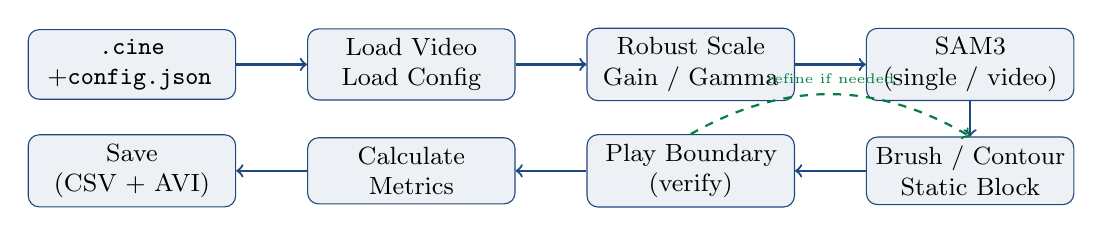
\begin{tikzpicture}[
      node distance = 0.45cm and 0.9cm,
      box/.style = {draw=myblue, rounded corners=4pt, fill=myblue!8,
                    text width=2.4cm, align=center, font=\small,
                    minimum height=0.8cm},
      arr/.style = {->, thick, myblue},
    ]
    \node[box] (A) {\texttt{.cine}\\+\texttt{config.json}};
    \node[box, right=of A] (B) {Load Video\\Load Config};
    \node[box, right=of B] (C) {Robust Scale\\Gain / Gamma};
    \node[box, right=of C] (D) {SAM3\\(single / video)};
    \node[box, below=of D] (E) {Brush / Contour\\Static Block};
    \node[box, left=of E]  (F) {Play Boundary\\(verify)};
    \node[box, left=of F]  (G) {Calculate\\Metrics};
    \node[box, left=of G]  (H) {Save\\(CSV + AVI)};

    \draw[arr] (A) -- (B);
    \draw[arr] (B) -- (C);
    \draw[arr] (C) -- (D);
    \draw[arr] (D) -- (E);
    \draw[arr] (E) -- (F);
    \draw[arr] (F) -- (G);
    \draw[arr] (G) -- (H);
    \draw[arr, dashed, mygreen] (F.north) to[bend left=30]
      node[above, font=\tiny, mygreen] {refine if needed} (E.north);
  \end{tikzpicture}}
  \end{center}

  \begin{columns}
    \column{0.48\linewidth}
      \textbf{Key design choices}
      \begin{itemize}
        \item All edits write to a single \texttt{plume\_masks} array — SAM3 and brush share the same state.
        \item Gain/Gamma affects both display \emph{and} the video sent to the model.
        \item Metrics use orifice-local $x=0$; \texttt{inner\_radius} from config ensures alignment.
      \end{itemize}
    \column{0.48\linewidth}
      \textbf{Output files}
      \begin{itemize}
        \item \texttt{*\_metrics.csv} — frame-wise spray metrics
        \item \texttt{*\_boundary\_points.csv} — boundary point cloud
        \item \texttt{*\_boundary.avi} — visualisation video
      \end{itemize}
  \end{columns}
\end{frame}

\end{document}
